\documentclass{article}
\usepackage{caption}
\usepackage{subcaption}

\usepackage{subcaption}
\usepackage{graphicx}

\usepackage{rotating}

\usepackage{helvet}
\renewcommand{\familydefault}{\sfdefault}

\begin{document}


\begin{sidewaysfigure}
     \centering
     \begin{subfigure}[b]{0.48\textwidth}
         \centering
         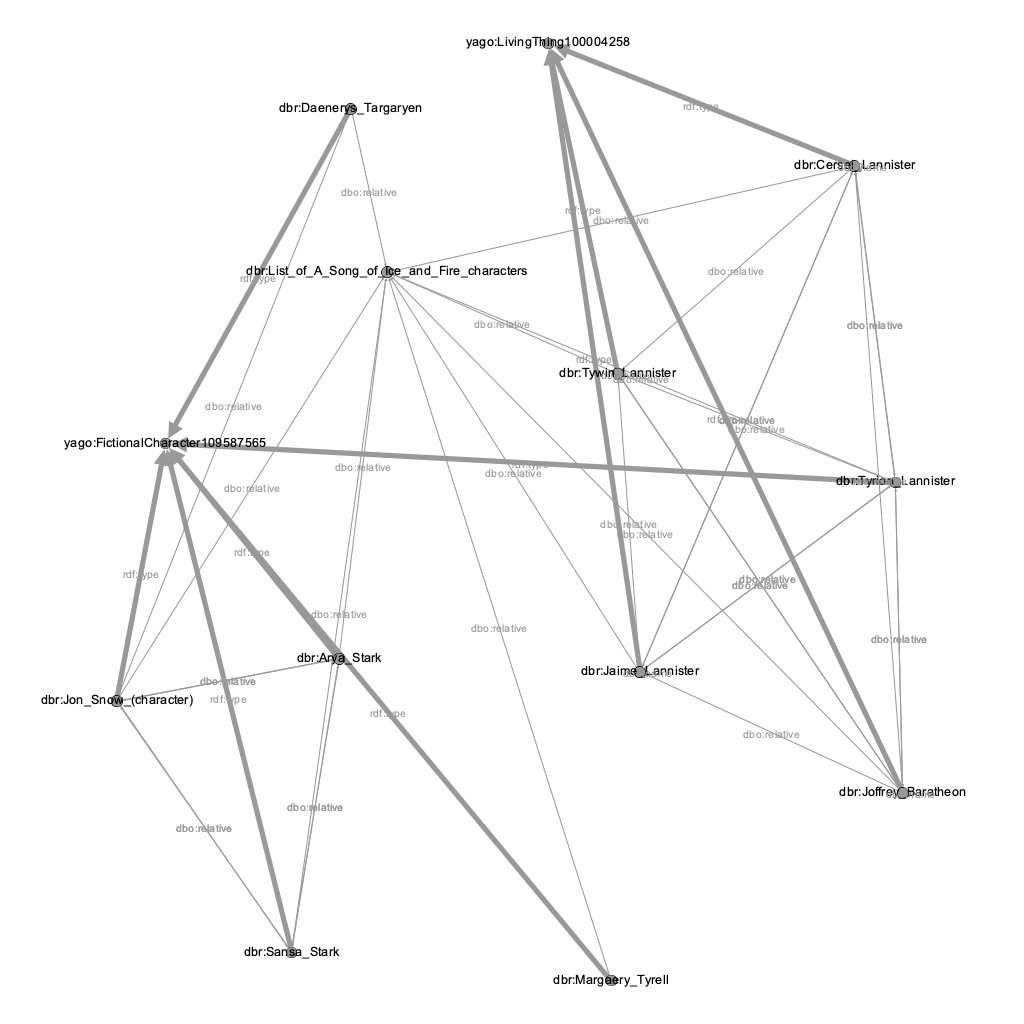
\includegraphics[width=\textwidth]{img/GotCharacters.png}
         \caption{}
         \label{fig:y equals x}
     \end{subfigure}
     \hfill
     \begin{subfigure}[b]{0.48\textwidth}
         \centering
         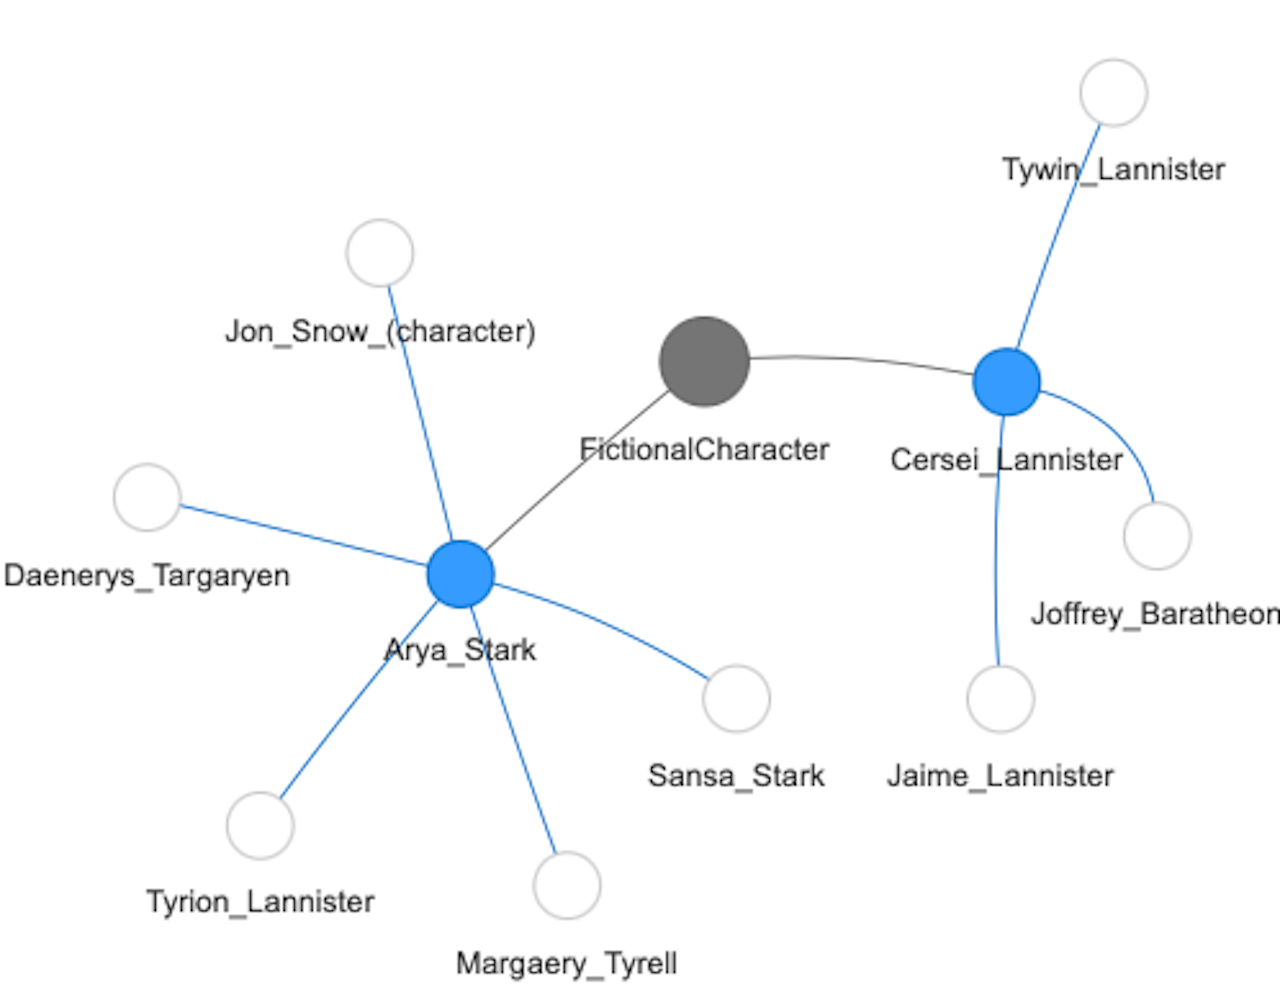
\includegraphics[width=\textwidth]{img/SemanticMapGot.png}
         \caption{}
         \label{fig:three sin x}
     \end{subfigure}
   %\caption{Three simple graphs}
    \label{fig:three graphs}
\end{sidewaysfigure}

\end{document}